\documentclass{article}
\usepackage{siunitx}
\usepackage{setspace}
\usepackage{gensymb}
\usepackage{xcolor}
\usepackage{caption}
%\usepackage{subcaption}
%\doublespacing
\singlespacing 
\usepackage[none]{hyphenat}
\usepackage{amssymb}
%\usepackage{relsize}
\usepackage[cmex10]{amsmath}
\usepackage{mathtools}
\usepackage{amsmath}
\usepackage{commath}
%\usepackage{amsthm}
%\interdisplaylinepenalty=2500
%\savesymbol{iint}
%\usepackage{txfonts}
%\restoresymbol{TXF}{iint}
%\usepackage{wasysym}
\usepackage{amsthm}
\usepackage{mathrsfs}
\usepackage{txfonts}
\let\vec\mathbf{}
%\usepackage{stfloats}
\usepackage{float}
\usepackage{cite}
\usepackage{cases}
\usepackage{subfig}
%\usepackage{xtab}
\usepackage{longtable}
\usepackage{multirow}
%\usepackage{algorithm}
\usepackage{amssymb}
%\usepackage{algpseudocode}
\usepackage{enumitem}
\usepackage{mathtools}
%\usepackage{eenrc}
%\usepackage[framemethod=tikz]{mdframed}
\usepackage{listings}
\usepackage{listings} 
\usepackage[latin1]{inputenc} 
%% \usepackage{color} 
%% \usepackage{array} 
%% \usepackage{longtable} 
%% \usepackage{calc} 
%% \usepackage{multirow} 
%% \usepackage{hhline} 
%% \usepackage{ifthen} 
%% %optionally (for landscape tables embedded in another document): 
%% \usepackage{lscape} 
\usepackage{titling}
%\usepackage{fulbigskip}
\usepackage{tikz}
\usepackage{graphicx}
\graphicspath{{/Internal storage/Download/fwc/figs}}
\begin{document} 
\title{CLASS 9\\10.CIRCLES}
\date{}
\maketitle
\section{EXERCISE 1}
\begin{enumerate}
\item $AD$ is a diameter of a circle and $AB$ is a chord. If $AD = 34 cm$, $AB = 30 cm$, the distance of $AB$ from the centre of the circle is:
\begin{enumerate}
\item 17cm
\item 15cm
\item 4cm
\item 8cm
\end{enumerate}
\item In Fig. \ref{fig:10.3}, if $OA = 5cm, AB = 8cm$ and $OD$ is perpendicular to $AB$, then $CD$ is equal to:
\begin{figure}[H]
\centering
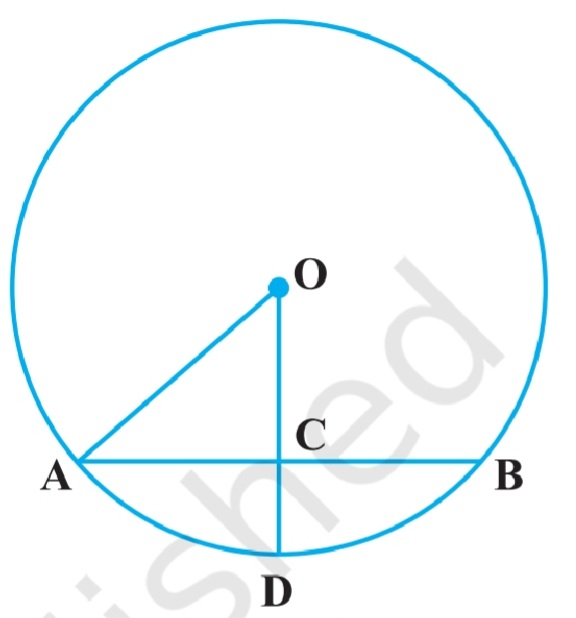
\includegraphics[width=\columnwidth]{figs/10.3.jpg}
\caption{}
\label{fig:10.3}
\end{figure}
\begin{enumerate}
\item 2cm
\item 3cm
\item 4cm
\item 5cm
\end{enumerate}
\item If $AB = 12 cm, BC = 16 cm$ and $AB$ is perpendicular to $BC$, then the radius of the circle passing through the points $\vec{A},\vec{B}$ and $\vec{C}$ is:
\begin{enumerate}
\item 6cm
\item 8cm
\item 10cm
\item 12cm
\end{enumerate}
\item In Fig. \ref{fig:10.4}, if $\angle ABC = 20\degree$ , then $\angle AOC$ is equal to: 
\begin{figure}[H]
\centering
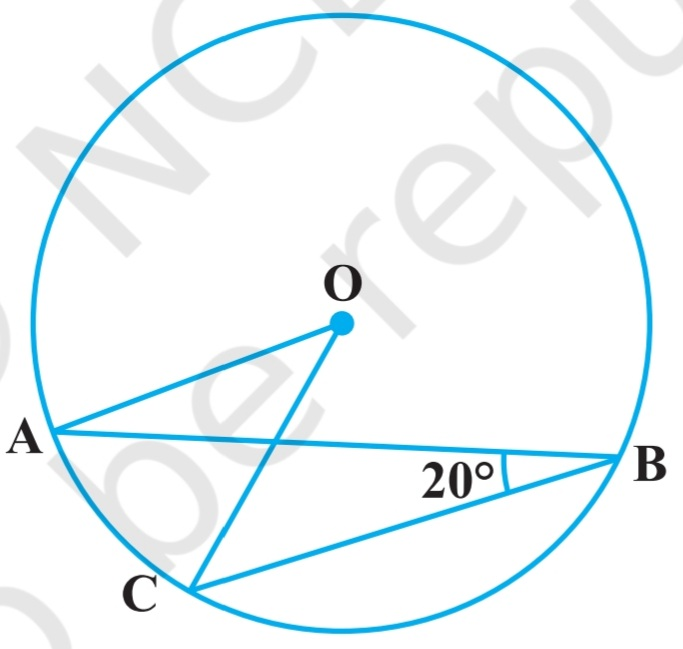
\includegraphics[width=\columnwidth]{figs/10.4.jpg}
\caption{}
\label{fig:10.4}
\end{figure}
\begin{enumerate}
\item $20\degree$
\item $40\degree$
\item $60\degree$
\item $10\degree$
\end{enumerate}
\item In Fig. \ref{fig:10.5}, if $AOB$ is a diameter of the circle and $AC = BC$,then $\angle CAB$ is equal to:
\begin{figure}[H]
\centering
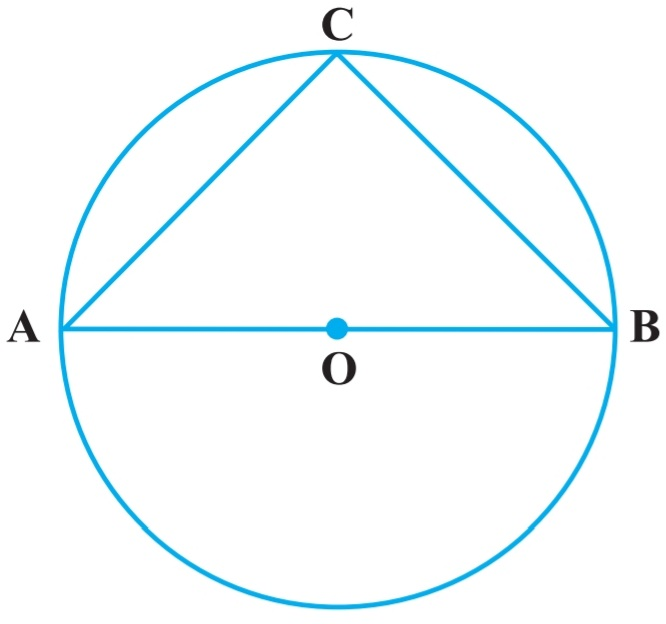
\includegraphics[width=\columnwidth]{figs/10.5.jpg}
\caption{}
\label{fig:10.5}
\end{figure}
\begin{enumerate}
\item $30\degree$
\item $60\degree$
\item $90\degree$
\item $45\degree$
\end{enumerate}
\item In Fig. \ref{fig:10.6}, if $\angle OAB = 40\degree$ , then $\angle ACB$ is equal to:  
\begin{figure}[H]
\centering
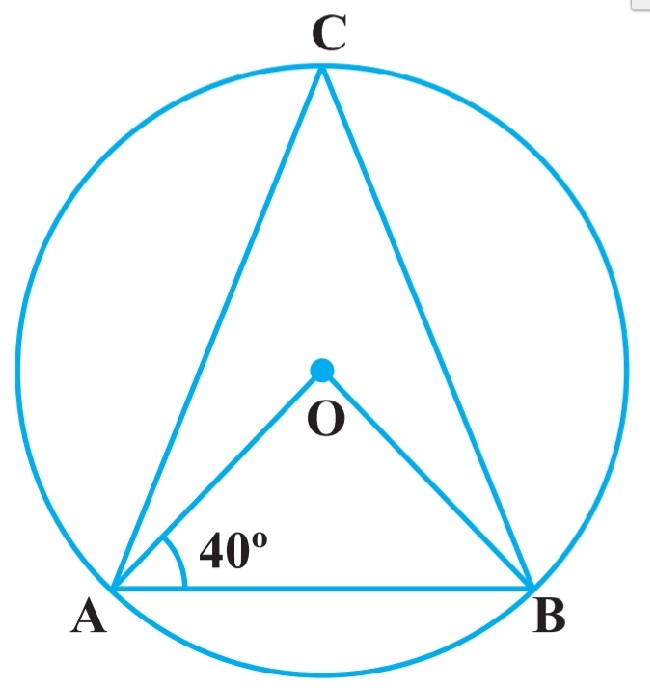
\includegraphics[width=\columnwidth]{figs/10.6.jpg}
\caption{}
\label{fig:10.6}
\end{figure}
\begin{enumerate}
\item $50\degree$
\item $40\degree$
\item $60\degree$
\item $70\degree$
\end{enumerate}
\item In Fig. \ref{fig:10.7}, if $\angle DAB = 60\degree , \angle ABD = 50\degree$ , then $\angle ACB$ is equal to:
\begin{figure}[H]
\centering
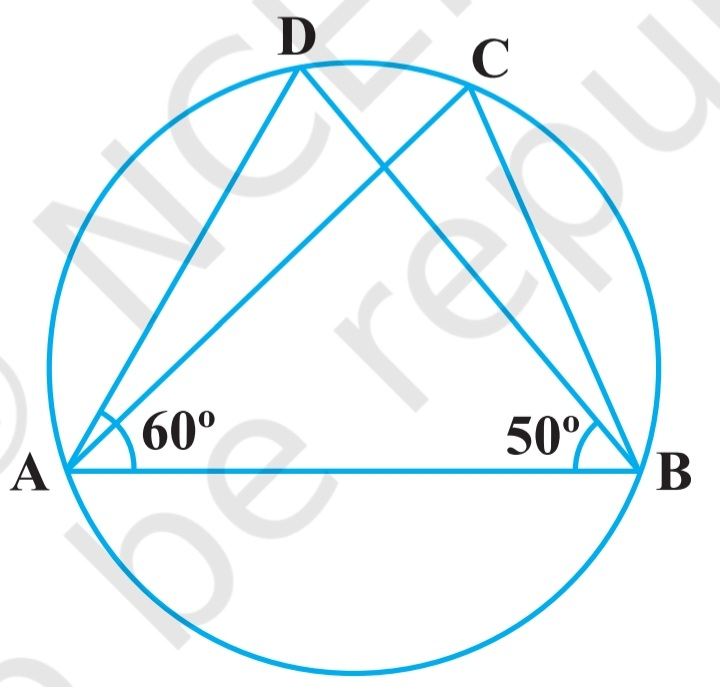
\includegraphics[width=\columnwidth]{figs/10.7.jpg}
\caption{}
\label{fig:10.7}
\end{figure}
\begin{enumerate}
\item $60\degree$
\item $50\degree$
\item $70\degree$
\item $80\degree$
\end{enumerate}
\item $ABCD$ is a cyclic quadrilateral such that $AB$ is a diameter of the circle circumscribing it and $\angle ADC = 140\degree$ , then $\angle BAC$ is equal to:
\begin{enumerate}
\item $80\degree$
\item $50\degree$
\item $40\degree$
\item $30\degree$
\end{enumerate}
\item In Fig. \ref{fig:10.8}, $BC$ is a diameter of the circle and $\angle BAO = 60\degree$. Then $\angle ADC$ is equal to:
\begin{figure}[H]
\centering
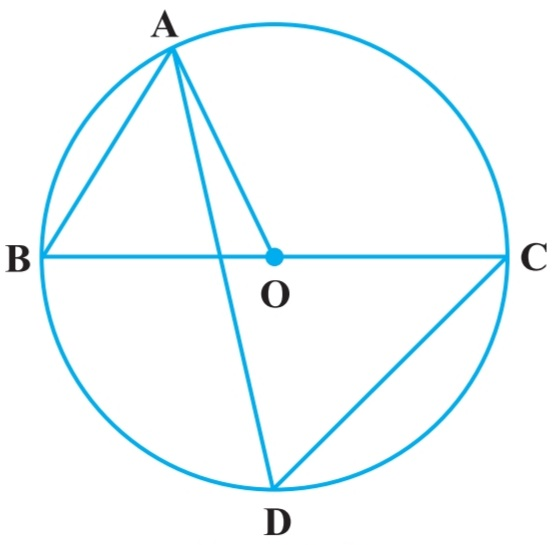
\includegraphics[width=\columnwidth]{figs/10.8.jpg}
\caption{}
\label{fig:10.8}
\end{figure}
\begin{enumerate}
\item $30\degree$
\item $45\degree$
\item $60\degree$
\item $120\degree$
\end{enumerate}
\item In Fig. \ref{fig:10.9}, $\angle AOB = 90\degree$ and $\angle ABC = 30\degree$ , then $\angle CAO$ is equal to:            
\begin{figure}[H]
\centering
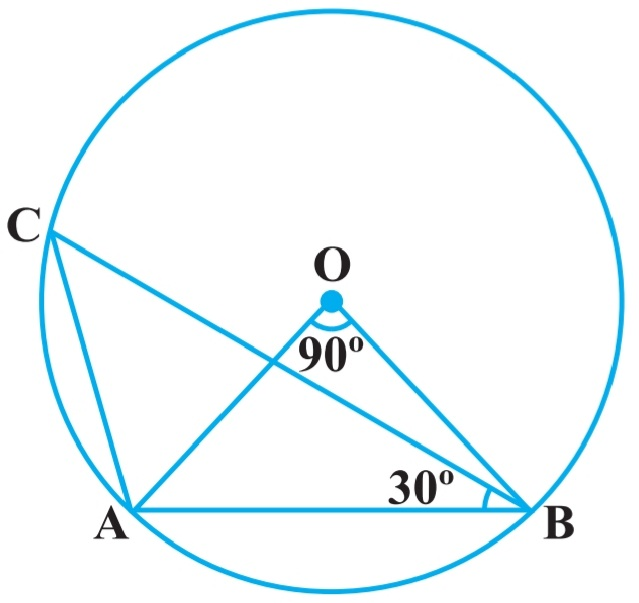
\includegraphics[width=\columnwidth]{figs/10.9.jpg}
\caption{}
\label{fig:10.9}
\end{figure}
\begin{enumerate}
\item $30\degree$
\item $45\degree$
\item $90\degree$
\item $60\degree$
\end{enumerate}
\end{enumerate}
\end{document}
